\documentclass{cta-author}

\makeatletter
\renewcommand\maketitle{\par%
  \begingroup
  \renewcommand\footnoterule{\begingroup\leftskip\z@\noindent
  \rule{84mm}{0.5\p@}\vspace{8\p@}\endgroup}
    \iferratum\relax\thispagestyle{erratumpage}\else\thispagestyle{titlepage}\fi%
    \renewcommand\thefootnote{\@fnsymbol\c@footnote}%
    \global\@topnum\z@%Prevents figures from going at top of page.
    \@maketitle
  \endgroup
  \@afterindentfalse
  \@afterheading
  \begingroup
  \def\thefootnote{}
  \endgroup
  \global\let\maketitle\relax
  \global\let\@maketitle\relax}
\makeatother

\begin{document}

\title{INSTRUCTION TO AUTHORS}

\author{}

\address{}

\maketitle


\section{Instructions for the Control Theory and Applications (CTA) \LaTeX\ Template}

This latex class file is available for authors to prepare
the manuscript for the Institution of Engineering and
Technology (IET) Journals. It is assumed that the authors
are familiar with either plain \TeX, \LaTeX,\ \AmS-\TeX\ or
a standard latex set-up, hence only the essential points
are described in this document. For more details please see
the \textit{\LaTeX\ User's Guide} or \textit{The not so
short introduction to \LaTeXe}.

\section{Installation}
Within the supplied set of files, \texttt{cta-author.cls} need to be copied into a directory
where tex looks for input files. The other files need to be kept as a reference while preparing your manuscript.
Please use pre-defined commands from \texttt{cta\_sample.tex} for title, authors, address, abstract, body etc.

\section{How to start using cta-author.cls}
Before you type anything that actually appears in the paper
you need to include a
\verb+\documentclass{cta-author}+ command at the
very beginning and then, the two commands that have to be
part of any latex document, \verb+\begin{document}+ at the
start and the \verb+\end{document}+ at the end of your
paper. The main structure of your document should be as
follows:

\begin{verbatim}
\documentclass{cta-author}
\usepackage[...]{packages}
\title{...}
\author{\au{S. Cheng$^{1,2}$} \au{J.C. Ji$^1$} \au{J. Zhou$^2$}}
%%\au{} represent author name

\address{\add{1}{.......}
%%\add{} represent author affiliation numbers
\add{2}{.......}
\email{........}}

\begin{abstract}
...............
\end{abstract}

\maketitle

\begin{document}

\section{....}
...
\subsection{....}
....
\end{document}
\end{verbatim}

\section{Table \& Figure environment}

To get the table caption use the command
\verb+\processtable{....}+, ensure to insert a brace \{
before \verb+\begin{tabular}+ and closing brace \} after
\verb+\end{tabular}+ (see below the table coding in detail).

\begin{verbatim}
\begin{table}[!t]
\processtable{Mobile robot parameters\label{tab1}}
{\begin{tabular}{@{\extracolsep{\fill}}lllll}\toprule
& & & Pioneer 2DX \\
Parameters & Pioneer 3DX & Pioneer 2DX & with load (4\,Kg) & Units\\\midrule
$\vartheta_{1}$ & \phantom{$-$}0.24089 & \phantom{$-$}0.3037 & \phantom{$-$}0.1992 & s \\
$\vartheta_{2}$ & \phantom{$-$}0.2424 & \phantom{$-$}0.2768 & \phantom{$-$}0.13736 & s \\
$\vartheta_{3}$ & $-$9.3603e$^{-4}$ & $-$4.018e$^{-4}$ & $-$1.954e$^{-3}$ & s.m/rad$^{2}$ \\
$\vartheta_{4}$ & \phantom{$-$}0.99629 & \phantom{$-$}0.9835 & \phantom{$-$}0.9907 \\
$\vartheta_{5}$ & $-$3.7256e$^{-3}$ & $-$3.818e$^{-3}$ & $-$1.554e$^{-2}$ & s/m \\
$\vartheta_{6}$ & \phantom{$-$}1.0915 & \phantom{$-$}1.0725 & \phantom{$-$}0.9866\\\botrule
\end{tabular}}{}
\end{table}
\end{verbatim}

\noindent Suppose, if you want to fit the table in double column, then use \verb+\fwprocesstable{....}+ as shown below:

\begin{verbatim}
\begin{table}[t]
\fwprocesstable{Coefficients and remainders for distribution KK ($k = 0.05$,
$v = 3$, $c_{1} = 1.5$, $c_{2} = 4.5$)}
{\begin{tabular*}{28pc}{@{\extracolsep{\fill}}lcc@{}}\toprule
$n$ & $a_{n}^{2}$ & $r_{k}(1)$\\\midrule
0 & 3.602576748428 & 1.493719547999\\
1 & 1.384791111989 & 0.108928436101\\
2 & 0.108600438794 & 0.000327997399\\
3 & 0.000275794597 & 0.000052202814\\
4 & 0.000018178621 & 0.000006407300\\\botrule
\end{tabular*}}{Table footnote}
\end{table}
\end{verbatim}

\noindent For figure caption use the following coding:

\begin{verbatim}
\begin{figure}[!t]
\centering{\includegraphics{fig2.eps}}
\caption{Consensus of trajectories of agents without a leader
\figfooter{a}{$\cos({\rm t})\omega_1=0.5$}
\figfooter{b}{$\omega_1=0$
{\rm Initial conditions and other parameters are chosen as $(p_i(0),q_i(0))=(0.2i,0.3i)$,
$c_{ij}=c_{ji}=0.2(i+j)$ and $m_i=0.1i (i,j=1,2,\ldots,6)$.}}
\label{fig2}}
\end{figure}
\end{verbatim}

\noindent The command \verb+\figfooter{}{}+ should be used to get the figure notes under figure caption.

\subsection{Equations}\label{sec3.10}

Equations are used in the same way as described in the \LaTeX\ manual.
Equations are numbered consecutively, with equation numbers
in parentheses flush right.\noindent

\vskip1pc
\noindent For example, if you type
\begin{verbatim}
\begin{equation}\label{eq1}
\int^{r_2}_0 F(r,\varphi){\rm d}r\,{\rm d}\varphi = [\sigma r_2/(2\mu_0)]
\int^{\infty}_0\exp(-\lambda|z_j-z_i|)\lambda^{-1}J_1 (\lambda r_2)J_0
(\lambda r_i\,\lambda {\rm d}\lambda)
\end{equation}
\end{verbatim}
then you will get the following output:
\begin{equation}\label{eq1}
\int^{r_2}_0 F(r,\varphi){\rm d}r\,{\rm d}\varphi = [\sigma r_2/(2\mu_0)]\int^{\infty}_0
\exp(-\lambda|z_j-z_i|)\lambda^{-1}J_1 (\lambda r_2)J_0 (\lambda r_i\,\lambda {\rm d}\lambda)
\end{equation}
\AmS-\LaTeX{} has several environments that
make it easier to typeset complicated multiline displayed equations. These are explained in the
\AmS-\LaTeX{} User Guide. A \verb+subequation+ environment is available to create equations with
sub-numbering of the equation counter. It takes one (optional)
argument to specify the way that the sub-counter should appear.


\subsection{Quotes and displayed text}
\label{sec3.11}

Quotes are indented from the left and right margins. There are various types of quotes,
short quote, long quote and display poetry.\vskip1pc

\noindent The coding for short quote is \verb+\begin{quote}...\end{quote}+.
\begin{quote}
   This is a short quotation.  It consists of a
   single paragraph of text.  See how it is formatted.
\end{quote}

\noindent The coding for long quote is \verb+\begin{quotation}...\end{quotation}+.

\begin{quotation}
   This is a longer quotation.  It consists of two
   paragraphs of text, neither of which are
   particularly interesting.

   This is the second paragraph of the quotation.  It
   is just as dull as the first paragraph.
\end{quotation}


\subsection{Listings}
\label{sec3.12}

Another frequently displayed structure is a list. There are various types of list
numbered, itemized and bulleted list.

\noindent The coding for bulleted list are as follows:

\begin{verbatim}
\begin{itemize}
\item Bulleted list 1
\item Bulleted list 2
\item Bulleted list 3
\end{itemize}
\end{verbatim}

\noindent The coding for numbered list are as follows:

\begin{verbatim}
\begin{enumerate}
\item Numbered list 1
\item Numbered list 2
\item Numbered list 3
\end{enumerate}
\end{verbatim}

\noindent The coding for description list are as follows:

\begin{verbatim}
\begin{description}
\item Description list 1
\item Description list 2
\item Description list 3
\end{description}
\end{verbatim}

\subsection{Enunciations like theorem, lemma etc.}
\label{sec3.13}

The \AmS-\LaTeX\ package for enunciations (amsthm.sty) has been already loaded in the class file.
For example, the command \verb+\newtheorem{theorem}{Theorem}+ has been already defined in the class file.

To get the theorem environment use the coding as:
\begin{verbatim}
\begin{theorem}
Theorem text. Theorem text. Theorem text.
Theorem text. Theorem text. Theorem text.
\end{theorem}
\end{verbatim}

Similarly, we can define for lemma, corollary, proposition, definition etc.

\subsection{Cross-referencing}
\label{sec3.14}

LATEX provides the following commands for cross referencing\vskip1pc

\noindent \verb+\label{marker}+, \verb+\ref{marker}+ and \verb+\pageref{marker}+\vskip1pc

\noindent where marker is an identifier chosen by the user. LATEX replaces \verb+\ref+ by
the number of the section, subsection, figure, table, or theorem after which
the corresponding \verb+\label+ command was issued. \verb+\pageref+ prints the page
number of the page where the \verb+\label+ command occurred.

\subsection{Citations}

Citations are made with the \verb+\cite+ command as usual. In this class file we have
used natbib.sty for cross references and reference style.

For bibliography the natbib package has been defined in the template as \verb+\usepackage{natbib}+.

For more details about natbib.sty can be found at
http://ctan.org/tex-archive/macros/latex/contrib/natbib/

\section*{Acknowledgements}

Acknowledgements and other unnumbered sections are created
using the \verb+\section*+ command:

\begin{verbatim}
\section*{Acknowledgment}
\end{verbatim}

\section*{Back Matter}

\subsection{References}
\label{sec3.18}

The reference entries can be \LaTeX\ typed bibliographies or generated through a BIB\TeX\ database.
BIB\TeX\ is an adjunct to \LaTeX\ that aids in the preparation of bibliographies. BIB\TeX\
allows authors to build up a database or collection of bibliography entries that may be used for many
manuscripts. They also save us the trouble of having to specify formatting. More details can be found
in the \textit{BIB\TeX\ Guide}. For clear understanding, please go through the documentation of \verb+IET_bst_HOWTO.pdf+.

For \LaTeX\ reference entries use the
\verb+\begin{thebibliography}..\end{thebibliography}+ environment (see below) to make references in your paper.
By default the class file will produce the unnumbered \LaTeX\ bibliography.

\begin{verbatim}
\begin{thebibliography}{99}

\bibitem{1}
Vicsek T., Czir\'{o}k A., Ben-Jacob E., Cohen I.: `Novel type of phase
transition in a system of self-driven particles', \textit{Phys.
Rev. Lett.}, 1995, \textbf{75}, pp.~1226--1229

\bibitem{2}
Jadbabaie A., Lin J., Morse A.S.: `Coordination of groups of
mobile autonomous agents using nearest neighbor rules', \textit{IEEE
Trans. Autom. Control}, 2003, \textbf{48}, pp.~988--1001

\bibitem{3}
Olfati-Saber R., Murray R.M.: `Consensus problems in networks
of agents with switching topology and time-delays', \textit{IEEE Trans.
Autom. Control}, 2004, \textbf{49}, pp.~1520--1533

\bibitem{4}
Ren W., Atkins E.: `Distributed multi-vehicle coordinated
control via local information exchange', \textit{Int. J. Robust
Nonlinear Control}, 2007, \textbf{17}, pp.~1002--1033

\bibitem{5}
Ren W.: `On consensus algorithms for double-integrator dynamics',
\textit{IEEE Trans. Autom. Control}, 2008, \textbf{53}, pp.~1503--1509

\end{thebibliography}
\end{verbatim}

\end{document}
